\documentclass[xcolor=table]{beamer}
\usepackage{fontspec}
\usepackage{natbib}
\usepackage{polyglossia} 
\usepackage[table]{xcolor}
\usepackage{gb4e} 
\usepackage{booktabs} 
\usepackage{multicol,multirow}
\usepackage{color}
%\usepackage{colortbl}
\usepackage{graphicx}
\usepackage{tikz}
\usetikzlibrary{arrows}



  \setmainfont[Mapping=tex-text]{Charis SIL}
\let\sfdefault\rmdefault
\newcommand{\racine}[1]{\begin{math}\sqrt{#1}\end{math}} 
\newcommand{\grise}[1]{\cellcolor{lightgray}\textbf{#1}} 
\usepackage{epsf}
   \newcommand{\ra}{$\Sigma_1$} 
\newcommand{\rc}{$\Sigma_3$} 
\newcommand{\ro}{$\Sigma$} 
\newfontfamily\phon[Mapping=tex-text,Ligatures=Common,Scale=MatchLowercase,FakeSlant=0.3]{Charis SIL} 
\newcommand{\rouge}[1]{{\color{red}#1}}
\newcommand{\bleu}[1]{{\color{blue}#1}}
 \newcommand{\ipa}[1]{{\phon #1}} %API tjs en italique
\newfontfamily\phondroit[Mapping=tex-text,Ligatures=Common,Scale=MatchLowercase]{Charis SIL} 
\newcommand{\ipapl}[1]{{\phondroit #1}} 
\newfontfamily\cn[Mapping=tex-text,Ligatures=Common,Scale=MatchUppercase]{MingLiU}%pour le chinois
\newcommand{\zh}[1]{{\cn #1}}

\begin{document} 
\begin{frame} 

\title{Sino-tibétain et panchronie} 

 \author{Guillaume Jacques, CNRS-CRLAO  }
\maketitle
 \end{frame} 

\begin{frame} 


\begin{itemize}[<+->]
\item hyperspécialisation
 \begin{tikzpicture}[font=\sffamily\small]
 \draw[triangle 60-triangle 60] (0,0) -- (4,0);
\end{tikzpicture}
dispersion

\item scepticisme
 \begin{tikzpicture}[font=\sffamily\small]
 \draw[triangle 60-triangle 60] (0,0) -- (5.4,0);
\end{tikzpicture}
spéculation

\end{itemize}
 \end{frame} 
 
\begin{frame} 

\begin{itemize}[<+->] 
\item Question fondamentale
\item Recherches empiriques (terrain et philologie)
\item Travail collaboratif
\end{itemize}
  \end{frame} 

\begin{frame} 
\frametitle{Question fondamentale}

\begin{itemize}[<+->] 
\item Quels sont les \bleu{principes généraux d'évolution des langues} (aussi bien en phonologie et morphologie qu'en syntaxe et en sémantique) et dans quelle mesure ces principes peuvent expliquer les tendances et universaux typologiques observées dans les langues du monde?
\item Linguistique \bleu{panchronique}
\item Comment contribuer de la façon la plus efficace à répondre à cette question?
\end{itemize}
  \end{frame} 
  
\begin{frame} 
\frametitle{Question fondamentale}

Famille \bleu{sino-tibétaine}

\begin{itemize}[<+->] 
\item Diversité considérable 
\item Profondeur historique
\item Documents anciens 
\item Travail de terrain possible
\end{itemize}
\end{frame} 

  
\begin{frame} 
\frametitle{Sous-question 1 (morphosyntaxe)}

\begin{itemize}[<+->]
\item Type \bleu{isolant} (chinois, birman): quelques traces de morphologie verbale dérivationnelle non-productives
\item Type \bleu{polysynthétique} (rgyalrong, kiranti): accord polypersonel, incorporation, morphologie gabaritique complexe et irrégulière 
\item Les langues isolantes ont-elles perdu leur morphologie?
\item Les langues polysynthétiques ont-elle récemment innové la leur et comment?
\item Dans quelle mesure ces données peuvent nous éclairer sur les principes généraux d'évolution de la morphologie verbale?
\end{itemize}

\end{frame} 


\begin{frame} 
\frametitle{Sous-question 2 (phonologie)}

\begin{itemize}[<+->]
\item Type `monosyllabique', structure syllabique simple (chinois, birman): C(R)V(C)
\item Structure syllabique complexe et mots polysyllabiques longs (rgyalrong)
\item Le type `monosyllabique' est-il le résultat d'une attrition phonétique et d'une simplification massive des groupes de consonnes?
\item Les mots longs et les groupes complexes des langues rgyalrong est-il innové à partir d'une langue à la structure syllabique simple? 
\end{itemize}

\end{frame} 



\begin{frame} 
\frametitle{Base empirique}

\begin{itemize}[<+->]
\item Manque de description fiable des langues rgyalronguiques et kiranties
\item Urgence d'une documentation détaillée (langues vulnérables ou en danger) 
\item Données \bleu{revérifiables} (corpus de textes / conversation)
\item Etude détaillée de quelques langues: \bleu{japhug} et \bleu{khaling}
\end{itemize}

\end{frame} 


 

\begin{frame} 
\frametitle{Japhug}
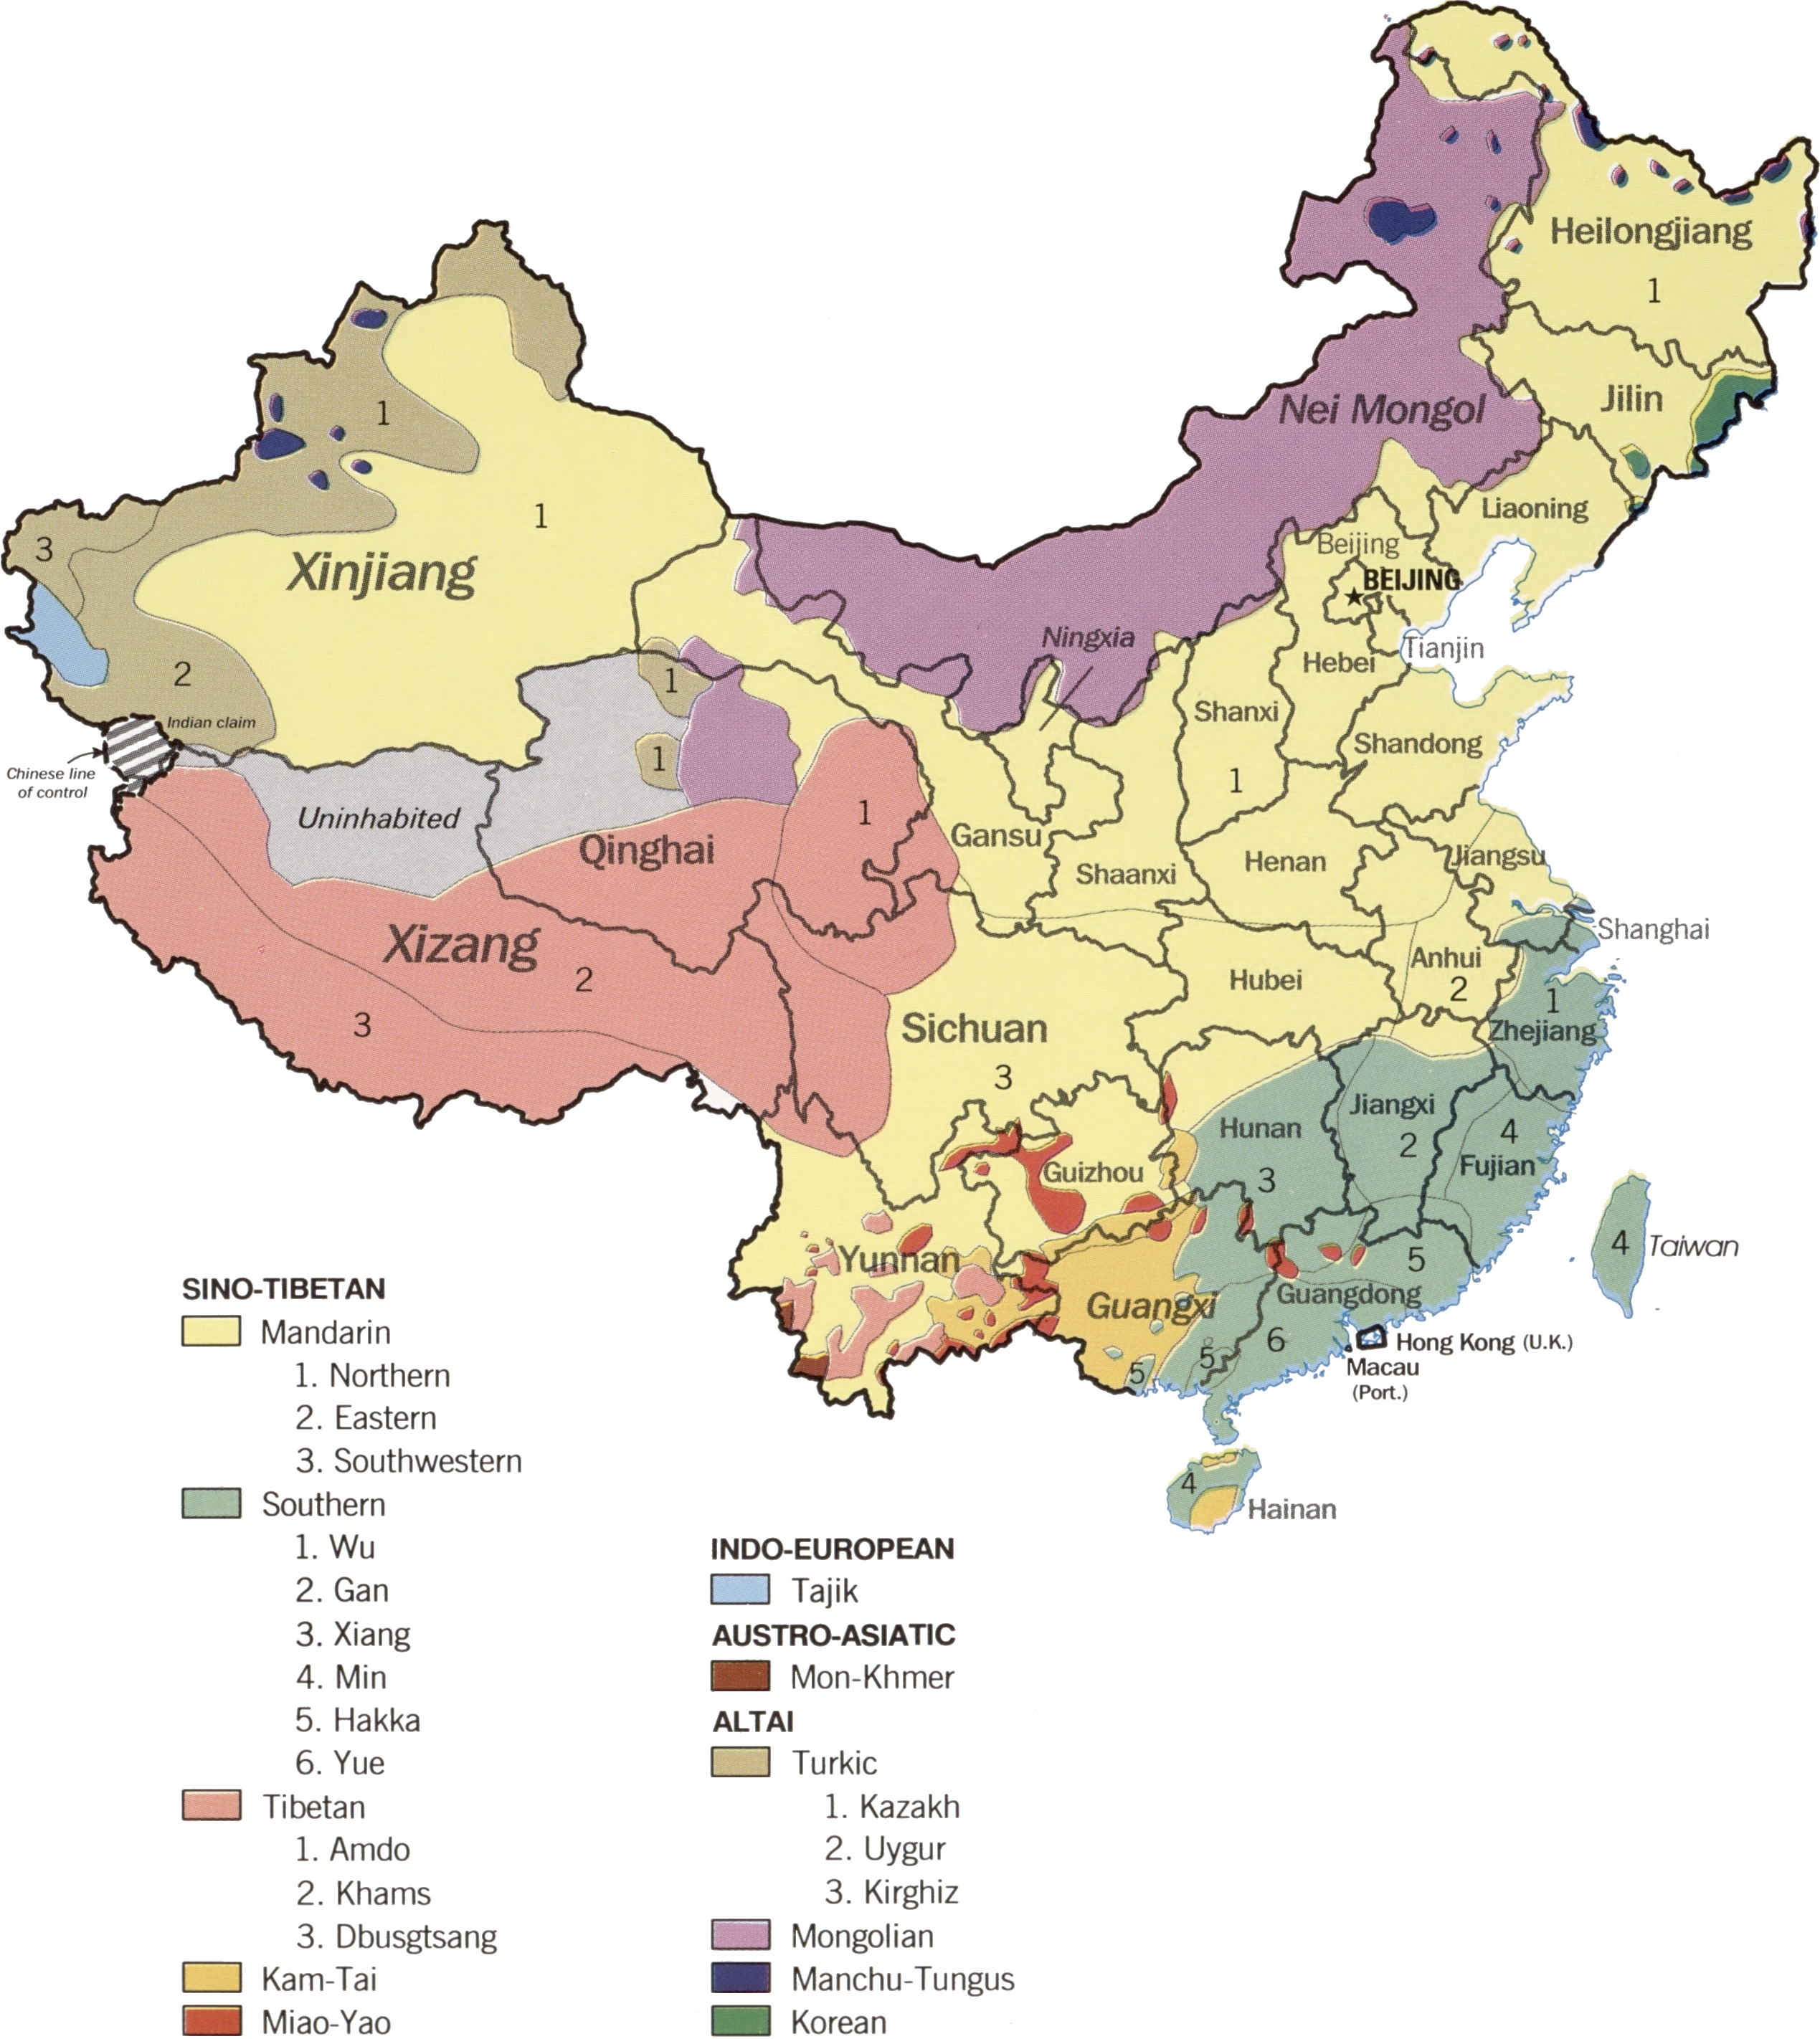
\includegraphics[width=0.8\textwidth]{chinalingmap.jpg} \centering
\end{frame} 

\begin{frame} 
\frametitle{Japhug}
Pour déterminer l'ancienneté de la morphologie verbale en japhug:
\begin{itemize}[<+->]
\item Evaluer au cas par cas pour chaque affixe si une hypothèse de grammaticalisation est possible
\item Méthode comparative
\end{itemize}
\end{frame} 



\begin{frame} 
\frametitle{Japhug}
Mise au jour de chemins de grammaticalisation non décrits dans d'autres langues:
\begin{itemize}[<+->]
\item incorporation
\item dénominal $\rightarrow$ voix (applicatif, antipassif, tropatif, causatif, passif)
\item causatif+passif $\rightarrow$ progressif
\item inverse $\rightarrow$ générique
\item dénominal+nominalisation $\rightarrow$  comitatif
\item origine des marqueurs de personne portemanteaux `sagittaux' (1$\rightarrow$2 et 2$\rightarrow$1)
\end{itemize}
\end{frame} 


\begin{frame} 
\frametitle{Japhug}
Caractéristiques typologiques rares:
\begin{itemize}[<+->]
\item Morphologie gabaritique préfixante dans une langue strictement verbe-finale
\item Marqueurs de mouvement associé et marqueurs directionnels distincts
\item Discours indirect hybride dans une langue à marquage personnel
\end{itemize}
\end{frame} 

\begin{frame} 
\frametitle{Khaling}

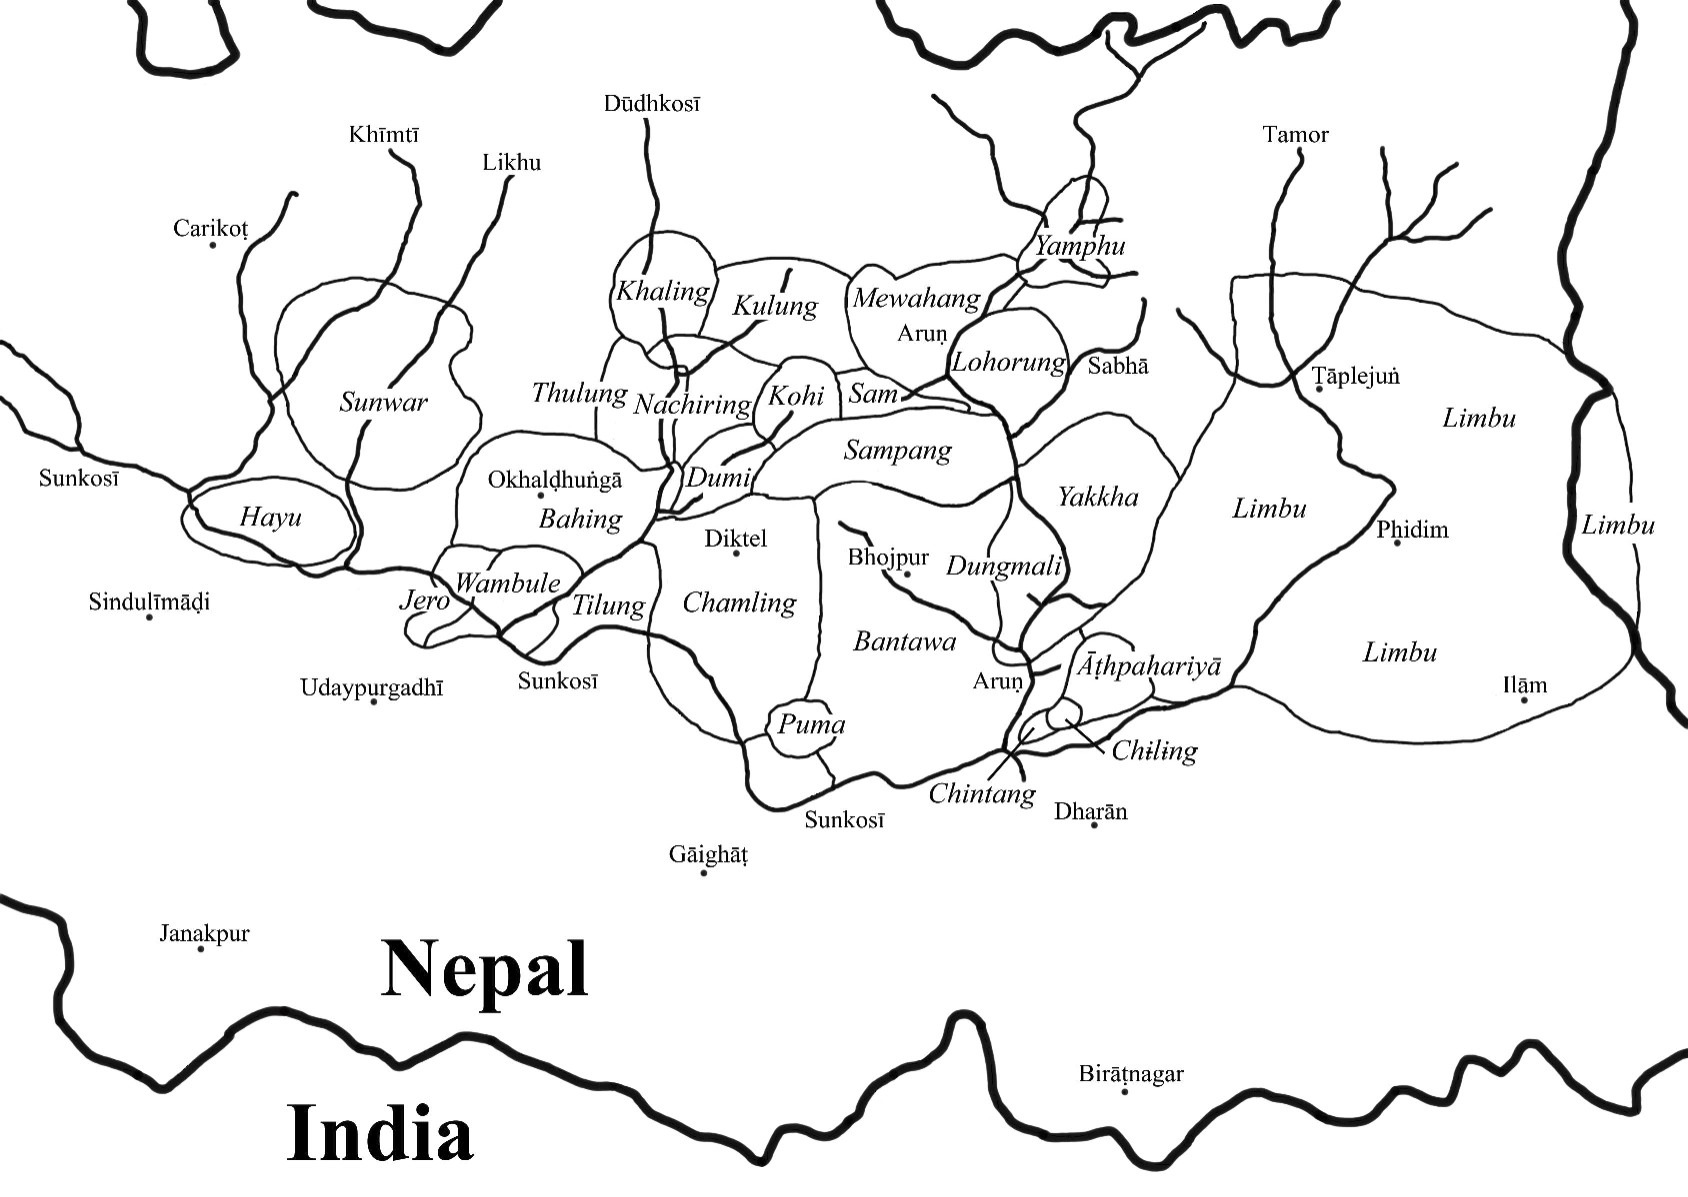
\includegraphics[width=1\textwidth]{Kirant.jpeg} 
\end{frame} 

\begin{frame} 
\frametitle{Khaling}
\begin{itemize}[<+->]
\item Génération des paradigmes 
\item Une curiosité: le démonstratif auditif
\item Mythologie locale 
\end{itemize}

\end{frame} 

\begin{frame} 
\frametitle{Travail collaboratif}
\begin{itemize}[<+->]
\item Travail avec informateurs
\item Intérêt de la documentation linguistique pour les locuteurs des langues étudiées

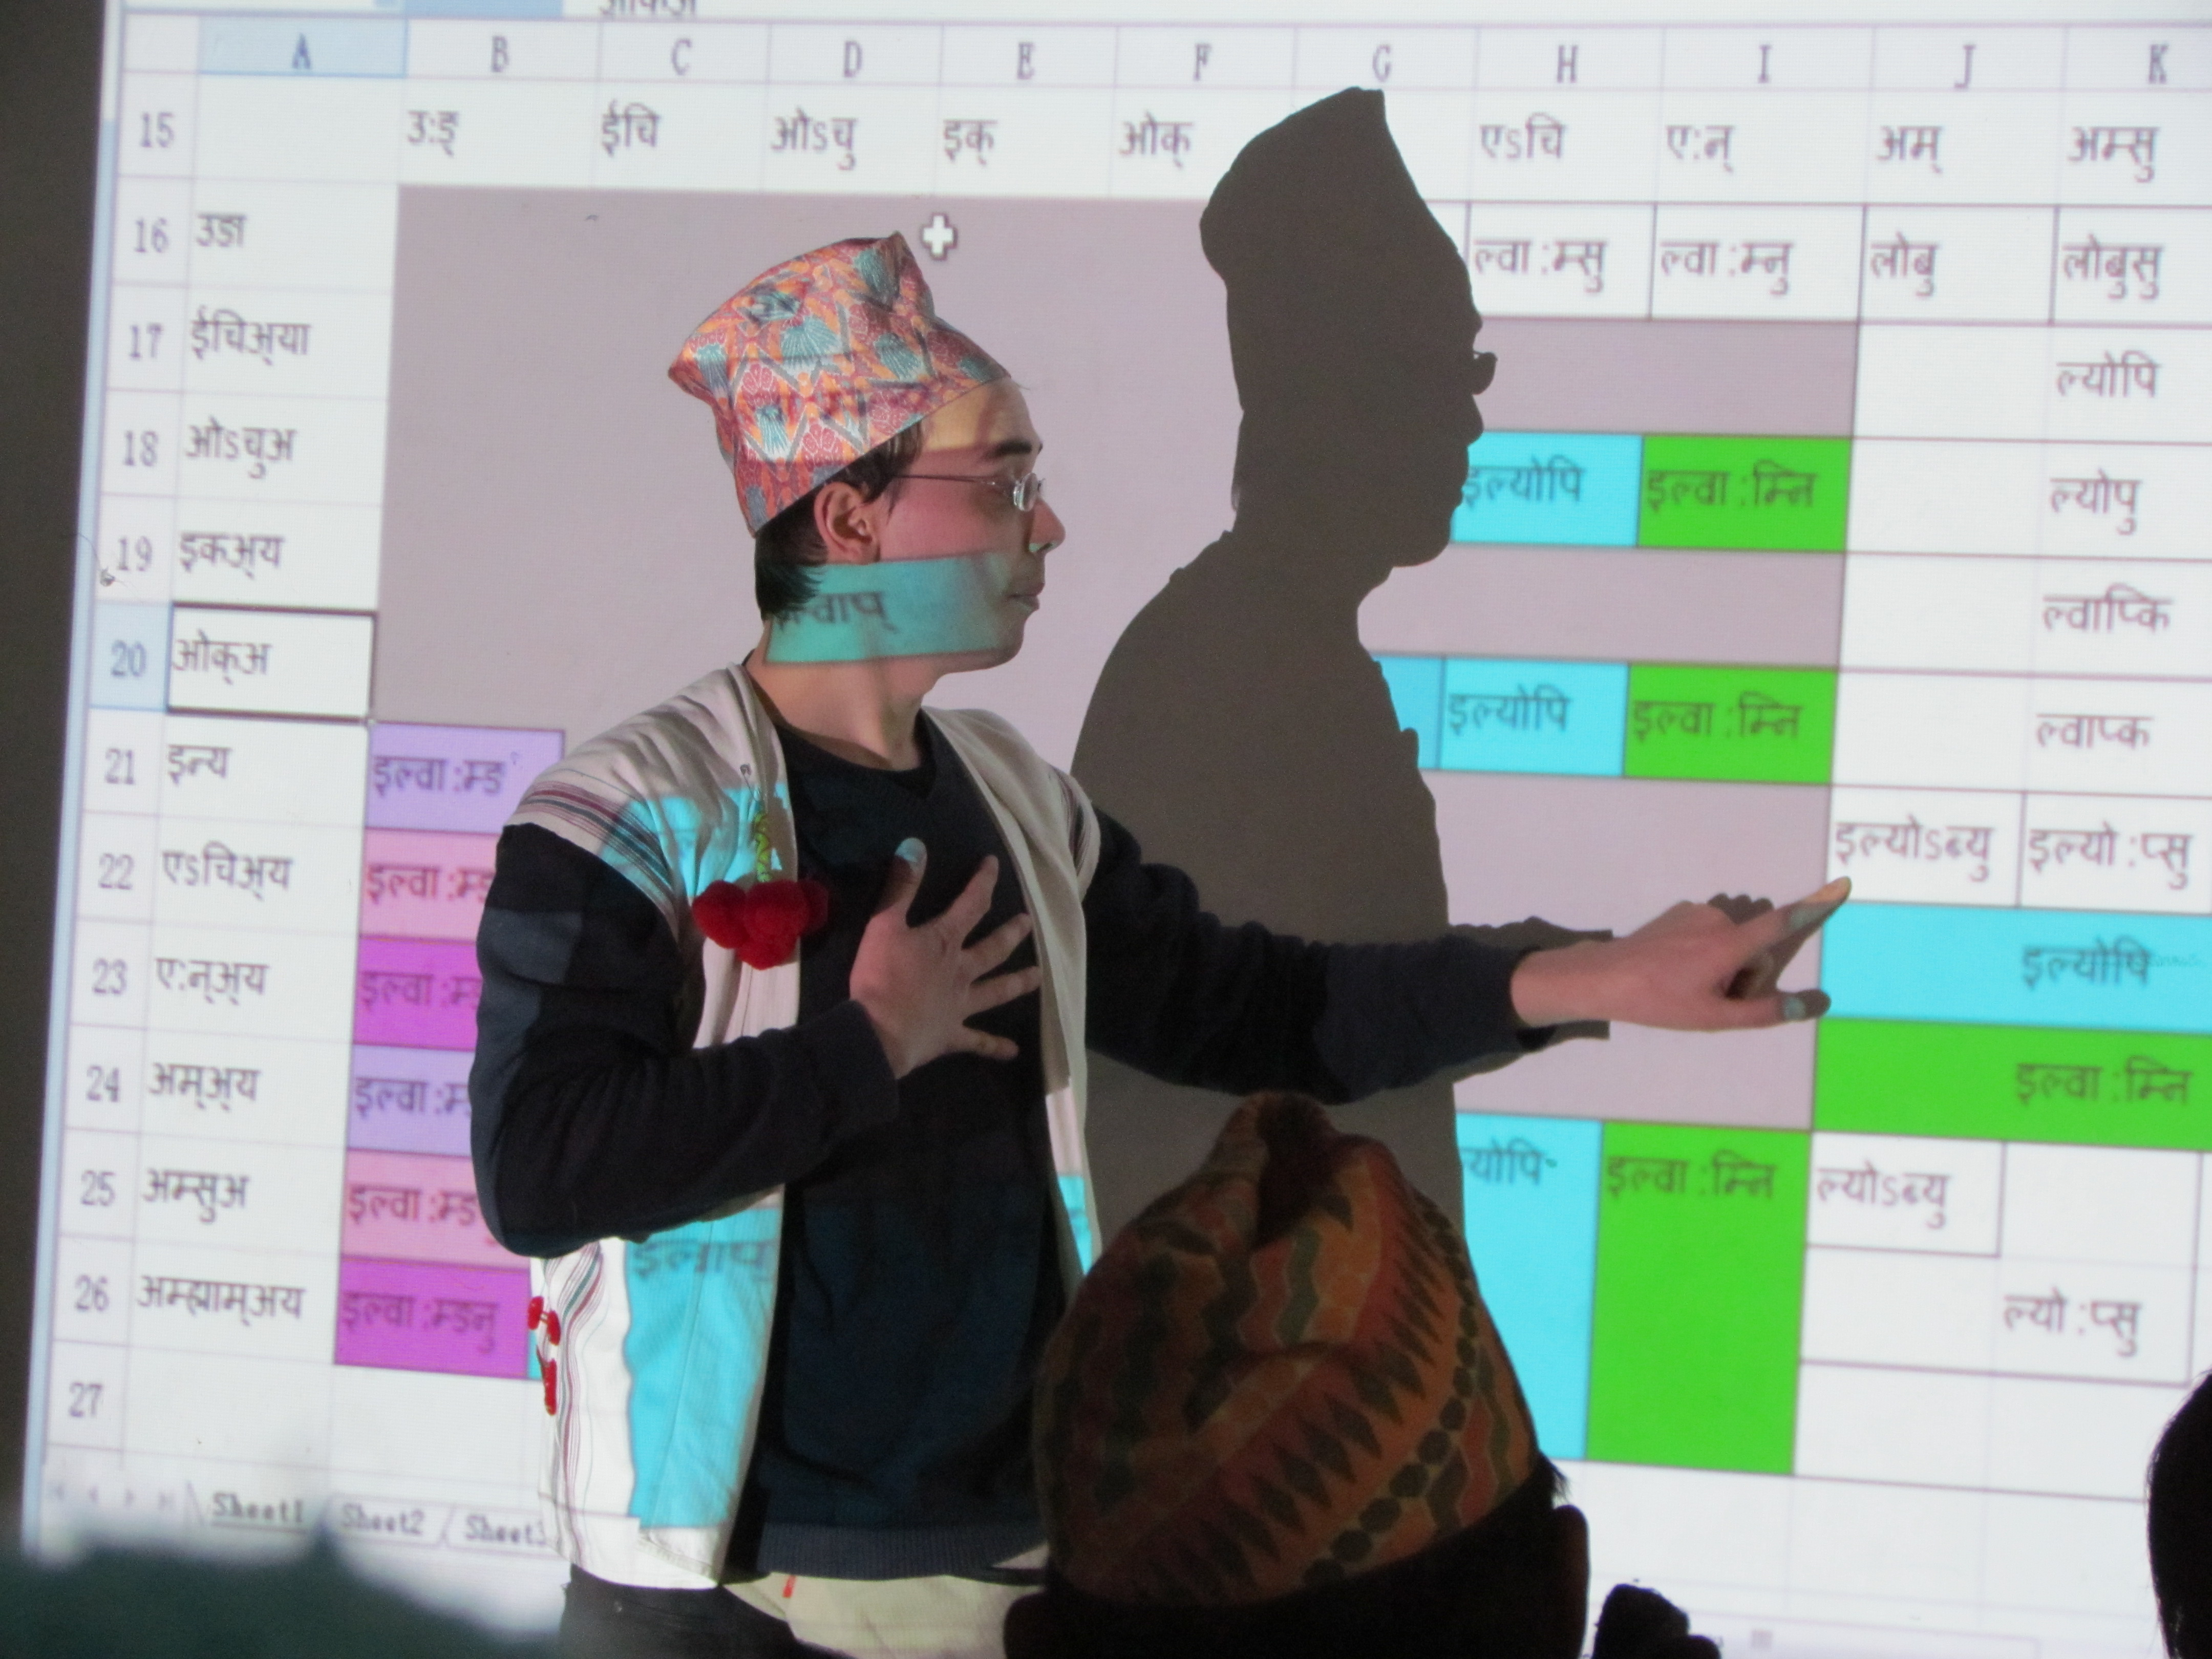
\includegraphics[width=0.5\textwidth]{hdr-image1.jpg}\centering
\end{itemize}

\end{frame} 

\begin{frame} 
\frametitle{Travail collaboratif}

\begin{itemize}[<+->]
\item Recherches de terrain collective
\item Rédaction en commun d'articles, mutualisation des compétences ($\Rightarrow$ quantité et qualité)
\item Formation d'étudiants ($\Rightarrow$ documentation d'autres langues)
\end{itemize}

\end{frame} 

\begin{frame}

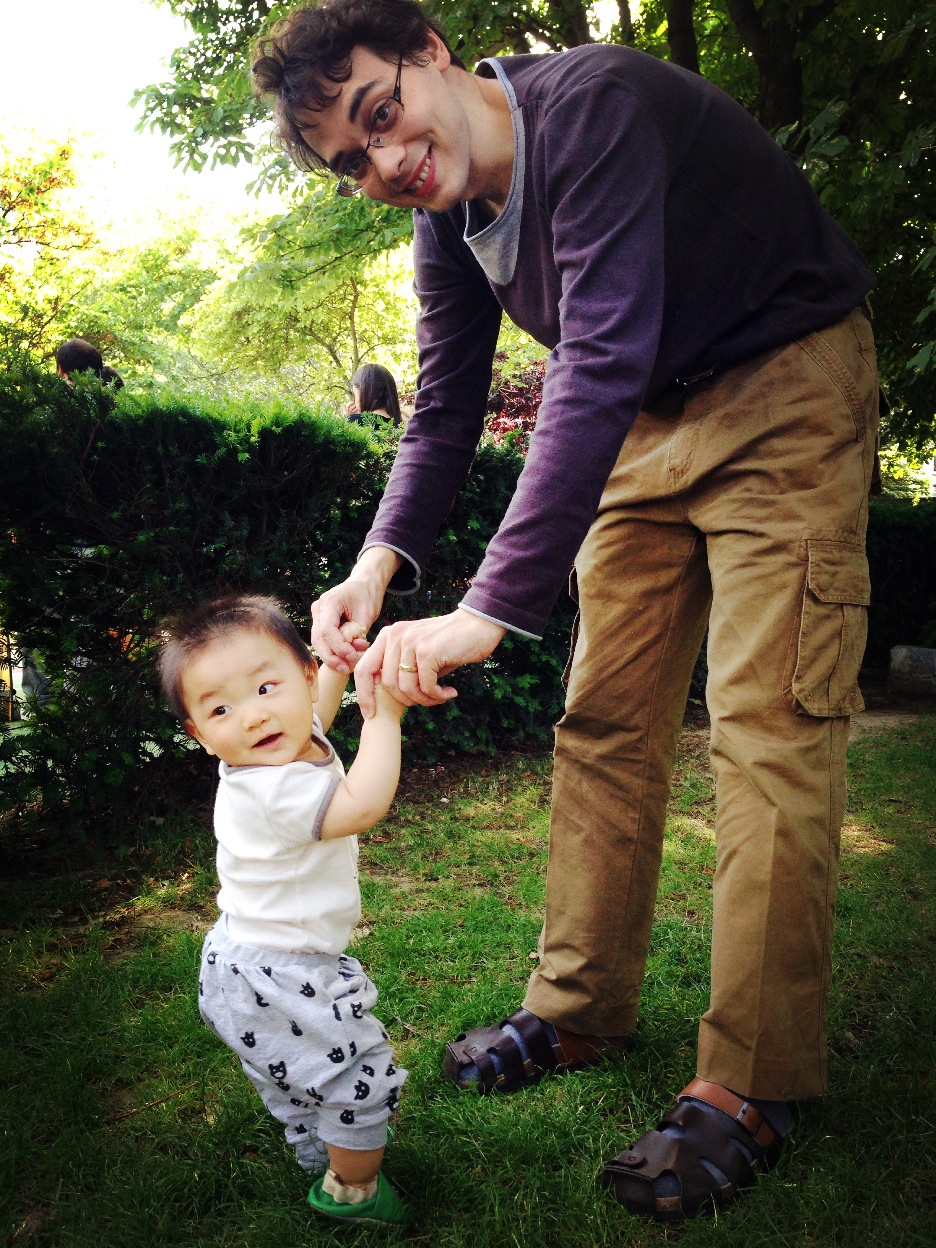
\includegraphics[width=0.6\textwidth]{archi.JPG} \centering
\end{frame}   
\end{document}


